\section{PERSIST-ACE}
\label{sec:method}

PERSIST-ACE is a local recovery layer for tool-using LLMs. As shown in
Figure~\ref{fig:framework}, its offline path compiles training failures into a
frozen Registry, while its online path detects a Functional Loop, admits one
grounded Recovery Card, and returns the resulting observation to the LLM.
Compilation is run independently for each benchmark; trajectories and Cards are
not pooled across benchmarks. PERSIST-ACE neither updates the base model nor
replaces its global planner.

\begin{figure*}[t]
\centering
\IfFileExists{figures/fig_persist_ace_pipeline.png}{%
  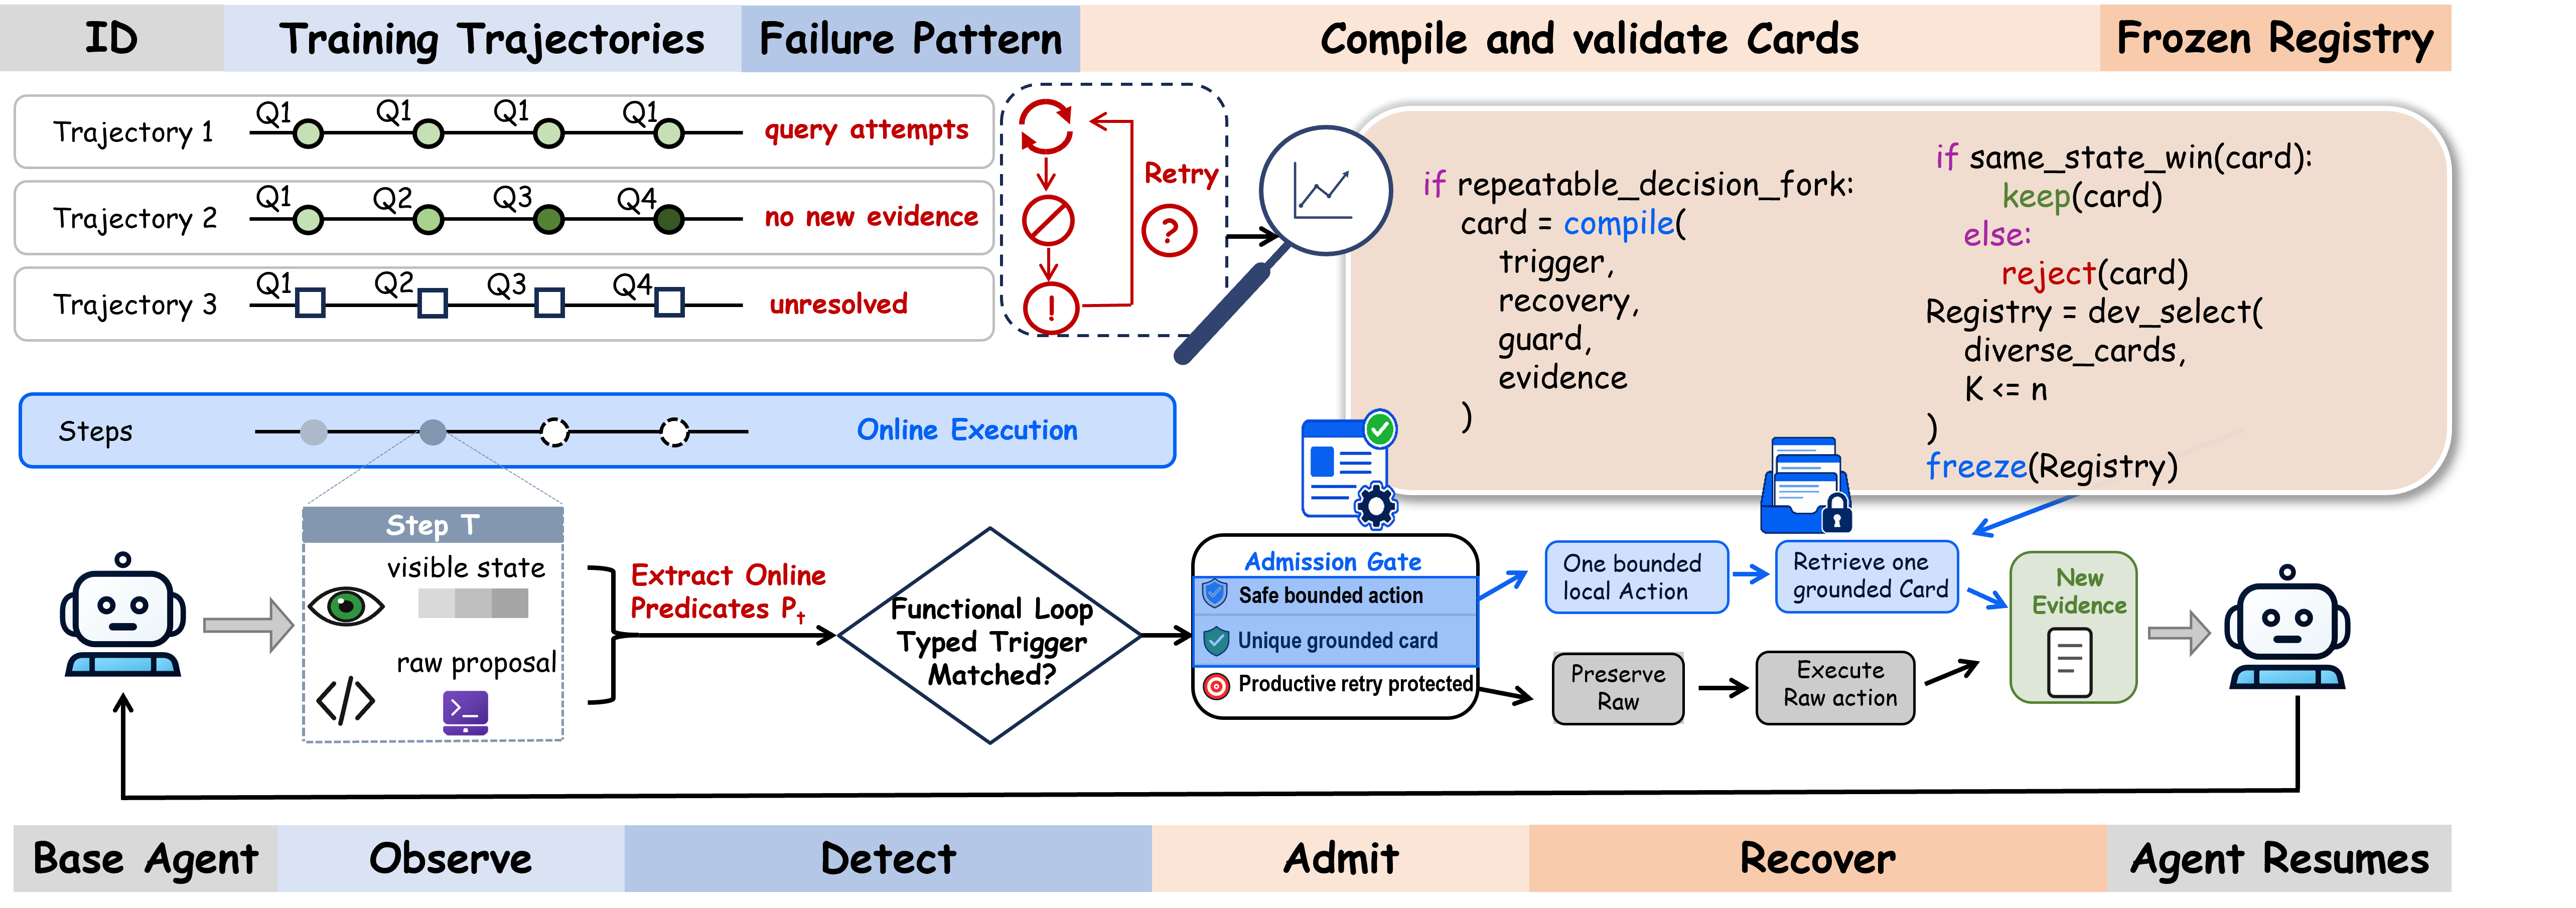
\includegraphics[width=0.97\textwidth]{figures/fig_persist_ace_pipeline.png}%
}{%
  \fbox{\parbox{0.95\textwidth}{\centering\small
  \textbf{Offline:} Raw training trajectories $\rightarrow$ suspicious
  pre-action states $\rightarrow$ effect/state clusters $\rightarrow$
  schema-grounded candidates $\rightarrow$ execution validation $\rightarrow$
  frozen benchmark-specific Registry
  \quad $\mid$ \quad
  \textbf{Online:} Raw proposal $+$ visible state $\rightarrow$
  trigger and guard checks $\rightarrow$ grounded recovery or Raw action}}
}
\caption{PERSIST-ACE compiles benchmark-specific training failures into a
frozen Registry. Online, it observes the state and Raw proposal, detects a
Functional Loop, admits a grounded and safe Card, executes one bounded
recovery, and returns control to the LLM.}
\label{fig:framework}
\end{figure*}

\subsection*{Offline Experience Compilation}

\textbf{Mine failure patterns.} The upper path of
Figure~\ref{fig:framework} starts from one benchmark's training trajectories.
At each pre-action prefix, $N$ recalls a no-progress state and $\kappa(e)$ tests
whether feedback-visible calls repeat the same unresolved effect. Only states
satisfying Eq.~\ref{eq:functional-loop} are Functional Loops. Other local
failures may inform recovery construction without being relabeled as loops. We
represent a candidate as
\begin{equation}
x_i=\left(s_i,a_i,e_i,\Delta E_i,\Delta S_i,u_i,\hat a_i,g_i,r_i\right),
\label{eq:candidate}
\end{equation}
where $\hat a_i$ is an executable replacement, $g_i$ its visible grounding
source, and $r_i$ a risk tag. Replacements may repair an argument, tool choice,
or blocked prerequisite, but cannot invent entities or relax user constraints.
Candidates are grouped by unresolved effect, requirement, action transition,
replacement, and grounding source.

\textbf{Compile and validate Cards.} Each supported group is compiled into a
Typed Recovery Card
\begin{equation}
c=(z_c,\phi_c,\psi_c,\rho_c,g_c,b_c,r_c),
\label{eq:card}
\end{equation}
where $z_c$ identifies the failure family, $\phi_c$ the trigger, $\psi_c$ the
abstention guards, $\rho_c$ the executable program, $g_c$ its grounding rule,
$b_c$ its budget, and $r_c$ its role and risk. Thus, a Card is a typed local
program rather than free-form advice. When snapshots are available, Raw and
Card actions are compared from the same state; otherwise we use paired or
repeated execution without claiming same-state evidence. Validation uses task
outcome and execution validity, while loop and cost measures remain
diagnostics.

\textbf{Freeze the Registry.} We reject candidates that require future or test
information, ambiguous entities, or constraint violations. Training-time
induction is protocol-constrained and LLM-assisted: a coding LLM may normalize
training failures and instantiate the fixed Card schema, but retention follows
the prescribed grounding, safety, validation, and development gates.
Researchers set this protocol without accessing test tasks or outcomes. Card
definitions, priorities, budgets, effect canonicalization, and controller
settings are frozen before test execution.

\subsection*{Online Selective Recovery}

\textbf{Observe and detect.} In the lower path of
Figure~\ref{fig:framework}, the LLM receives tool feedback and proposes Raw
action $a_t$. Observe exposes the visible history and state $s_t$: effects,
evidence changes, unresolved requirements, constraints, and the proposal.
Detect applies Eq.~\ref{eq:functional-loop}; $N=1$ recalls no progress and
$R_e=1$ confirms a repeated feedback-visible effect. It uses no future outcome.
A repeated tool name is insufficient, and detection alone does not authorize
intervention.

\textbf{Admit.} The controller next retrieves Cards whose trigger matches the
current Functional Loop family. Let the eligible set at step $t$ be
\begin{equation}
\begin{aligned}
\mathcal{C}_t=\{c\in\mathcal{R}:{}&\phi_c(s_t,a_t)=1
\land\psi_c(s_t,a_t)=0,\\
&b_c>0\land\operatorname{Unique}(g_c(s_t))=1,\\
&\operatorname{Safe}(\rho_c(s_t,a_t))=1\}.
\end{aligned}
\label{eq:eligible}
\end{equation}
where $\phi_c$ matches the state and effect, $\psi_c$ protects productive
retries, and $b_c$ is the remaining budget. Admission also requires unique
grounding and a schema-valid, constraint-preserving action. A frozen priority
order favors smaller changes, stronger grounding, validation support, and
lower risk. Recent progress, a productive retry, ambiguity, conflict, budget
exhaustion, or a failed safety check preserves the Raw proposal.

\textbf{Recover and resume.} For the highest-priority admitted Card
$c^\star$, the executed policy is
\begin{equation}
\pi_{\mathrm{ACE}}(s_t,a_t)=
\begin{cases}
\rho_{c^\star}(s_t,a_t), & \mathcal{C}_t\neq\varnothing,\\
 a_t, & \mathcal{C}_t=\varnothing,
\end{cases}
\label{eq:controller}
\end{equation}
The environment executes the bounded Card program or the Raw action and returns
a new observation. Control then returns to the LLM. Cards cannot invoke one
another without an intervening LLM proposal, and recovery does not guarantee
task success. Functional Loop detection locates an opportunity; admission
decides whether and how to act.
